
%%%%%%%%%%%%%%%%%%%%%%%%%%%%%%%%%%%%%%%%%%%%%%%%%%%%%%%
%%              Supplementary Content                %%
%%%%%%%%%%%%%%%%%%%%%%%%%%%%%%%%%%%%%%%%%%%%%%%%%%%%%%%
%------------------------------------------------
\section{Supplementary content}
%------------------------------------------------
\subsection{Hyperparameter tuning results}
%------------------------------------------------
\begin{frame}[t,noframenumbering]
	\frametitle{Hyperparameter tuning: other hyperparamters}
	\tikzstyle{background grid}=[draw, black!50,step=.5cm]
	%
	We can use StoMADS to solve such hyperparameter optimization problems \ifshowcitations\footpartcite{Khalil2021}\fi\\
	%
	\tikzstyle{background grid}=[draw, black!50,step=.5cm]
	\begin{tikzpicture}[remember picture, overlay] %show background grid, 
		% Put the graphic inside a node. This makes it easy to place the
		% graphic and to draw on top of it. 
		% The above right option is used to place the lower left corner
		% of the image at the (0,0) coordinate. 
		\node [inner sep=0pt,above right, opacity=1.0]  at (-0.01\textwidth,-0.7\textheight) (error) 
			{
				\only<1>{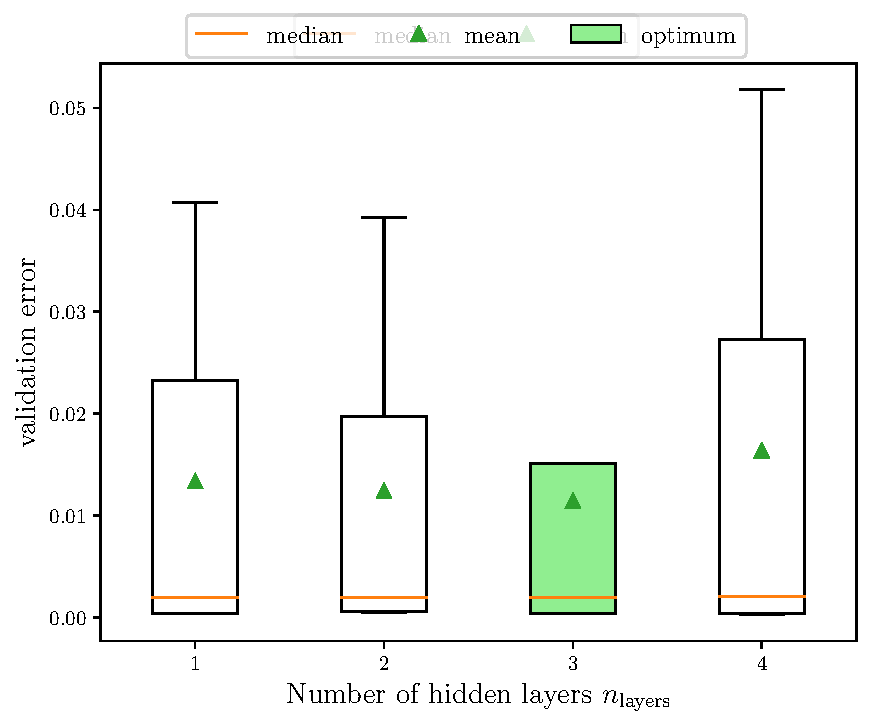
\includegraphics[width=0.5\textwidth]{box_plots/boxplot_n_layers_opt.pdf}}%
				\only<2>{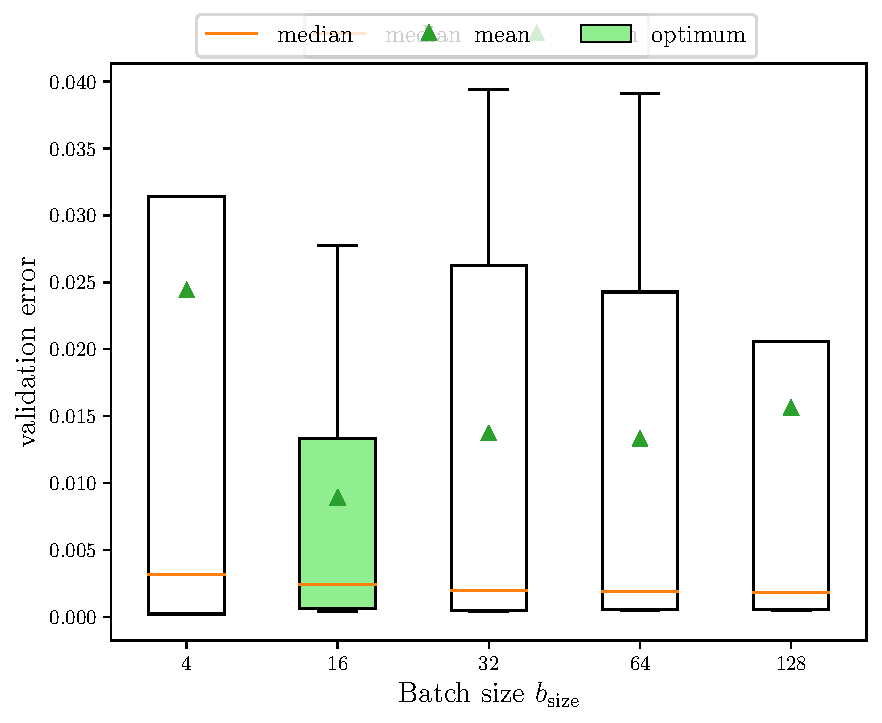
\includegraphics[width=0.5\textwidth]{box_plots/boxplot_batch_size_opt.pdf}}%
				\only<3>{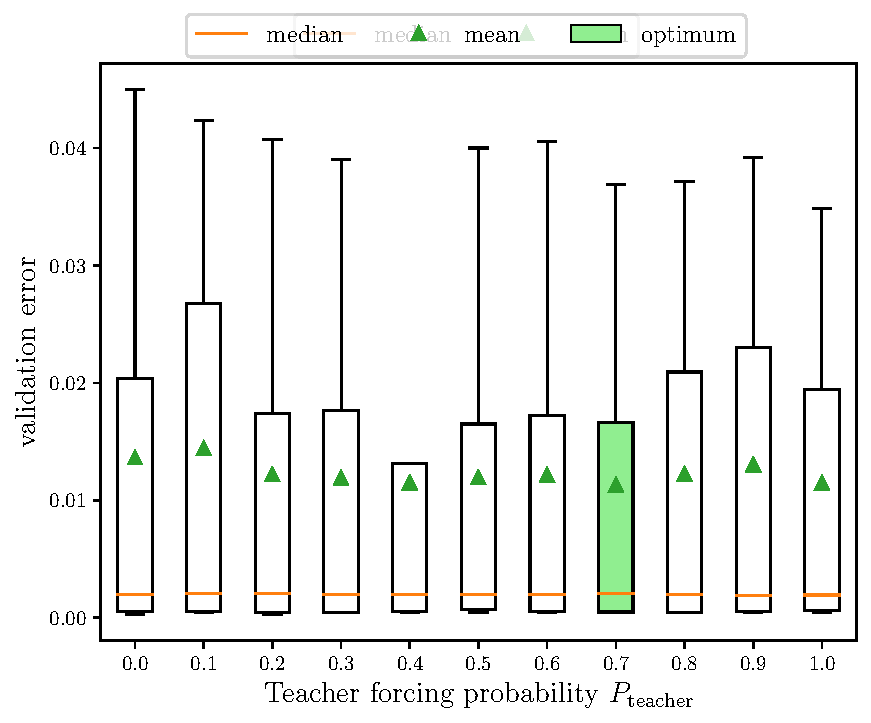
\includegraphics[width=0.5\textwidth]{box_plots/boxplot_teacher_forcing_opt.pdf}}%
				\only<4->{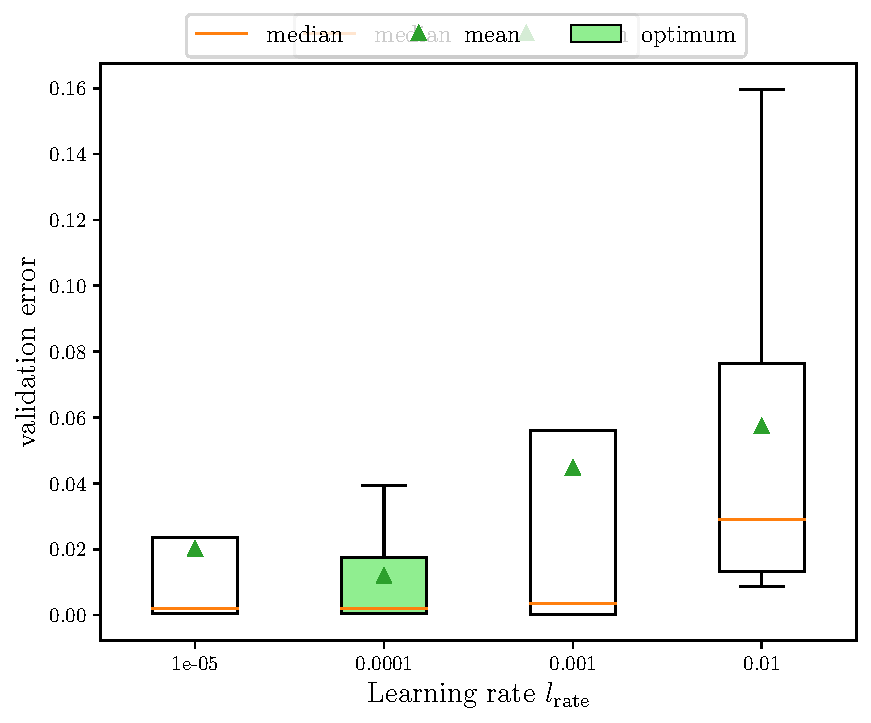
\includegraphics[width=0.5\textwidth]{box_plots/boxplot_learning_rate_opt.pdf}}%
			};
		\node [inner sep=0pt,above left, opacity=1.0]  at (1.01\textwidth,-0.7\textheight) (prediction) 
			{
				\only<1>{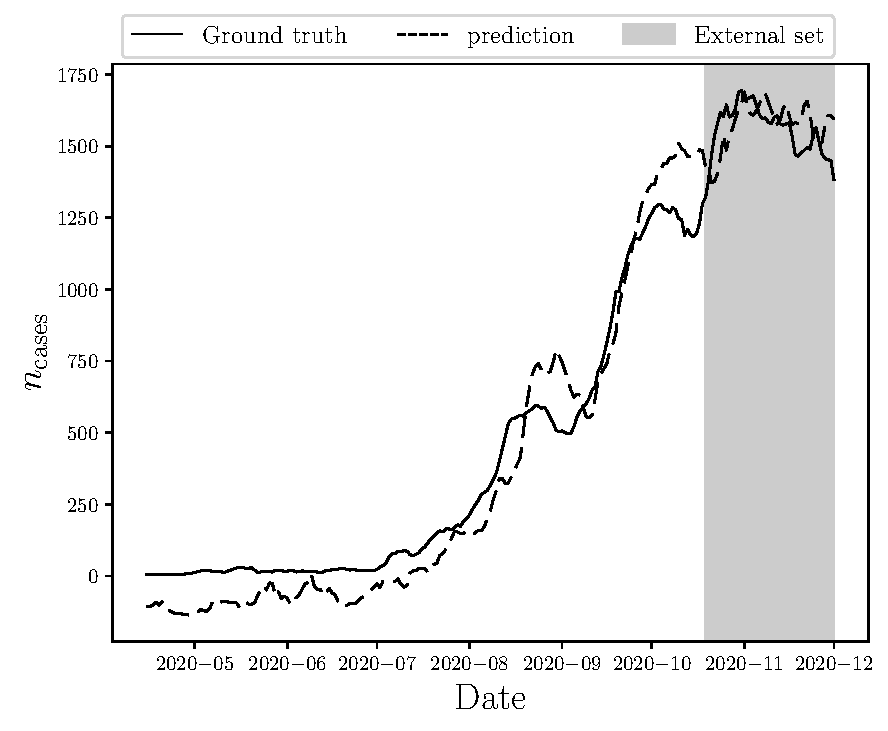
\includegraphics[width=0.5\textwidth]{models/final_model_n_layers.pdf}}%
				\only<2>{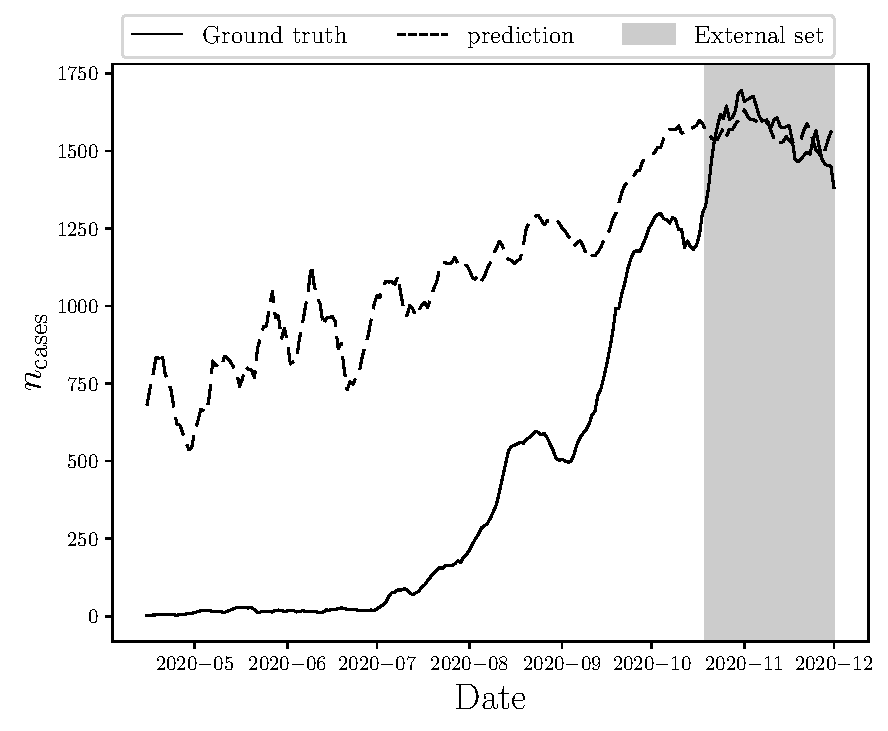
\includegraphics[width=0.5\textwidth]{models/final_model_batch_size.pdf}}%
				\only<3>{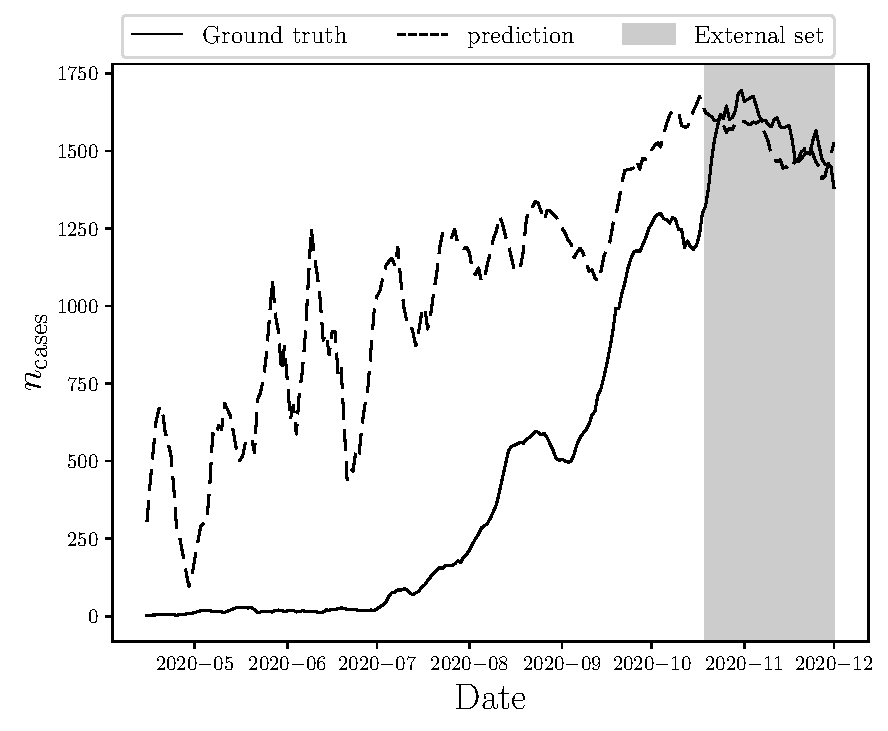
\includegraphics[width=0.5\textwidth]{models/final_model_teacher_forcing.pdf}}%
				\only<4->{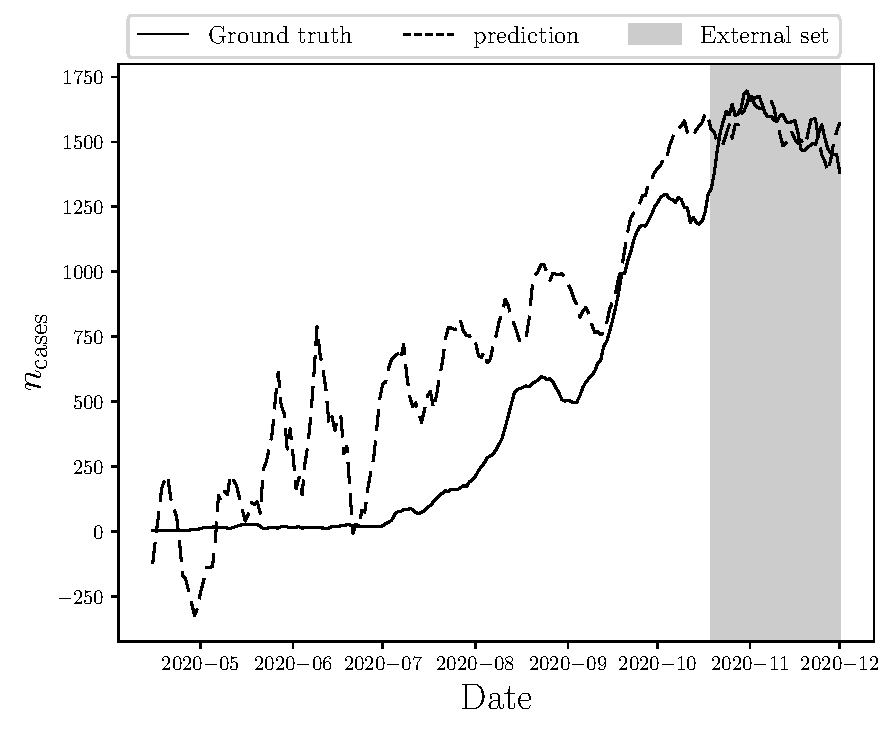
\includegraphics[width=0.5\textwidth]{models/final_model_learning_rate.pdf}}%
			};
		% show origin
		% \fill (0,0) circle (2pt);
	\end{tikzpicture}%
	%
	\vspace{-3em}
\end{frame}
\addtocounter{footnote}{-1}
%------------------------------------------------